\section{Gaussian Mixture Models}
K-means clustering is a hard-clustering, but in some cases soft-clustering provides a better model in practice. Gaussian mixture model assumes a simple \textbf{linear superposition} of Gaussian components, aimed at providing a richer class of density models than the single Gaussian. Let's consider a single sample case and it can be expressed as follows:
$$p(\mathbf{x})= \sum_{k=1}^{K}\pi_k\mathcal{N}(\mathbf{x}|\boldsymbol{\mu_k}, \boldsymbol{\Sigma}_k)$$
Let us introduce a $K$-dimensional binary random variable $\mathbf{z}$ having a 1-of-$K$ representation in which a particular element $z_k$ is equal to 1 and all other elements are 0. I will explain more about $\mathbf{z}$ later. It satisfied the following properties:
\begin{itemize}
	\item $z_k\in\{0,1\}$
	\item $\sum_kz_k=1$
\end{itemize}
The marginal distribution over $\mathbf{z}$ is specified in terms of the mixing coefficients $\pi_k$, such that 
$$p(z_k=1) = \pi_k$$
, where the mixing coefficients must satisfy
$$0\leq\pi_k\leq1$$
and 
$$\sum_{k=1}^{K}\pi_k = 1 $$
in order to be valid probabilities. We can also write pdf of $\mathbf{z}$ in a product of mixing coefficient because it is a 1-of-$K$ representaion.
$$p(\mathbf{z}) = \prod_{k=1}^{K}\pi_k^{z_k} = \pi_k \because z_k\in\{
0,1\}$$
Similarly, the conditional distribution of $\mathbf{x}$ given a particular $\mathbf{z}$ can be modeled to be a Gaussian distribution.
\begin{equation*}
p(\mathbf{x}|z_k=1) = \mathcal{N}(\mathbf{x}|\boldsymbol{\mu}_k, \boldsymbol{\Sigma}_k) 
\end{equation*}
Also can be represented in the form 
\begin{align*}
p(\mathbf{x}|\mathbf{z}) &= \prod_{k=1}^{K}\mathcal{N}(\mathbf{x}|\boldsymbol{\mu}_k, \boldsymbol{\Sigma}_k)^{z_k}\\
& = \mathcal{N}(\mathbf{x}|\boldsymbol{\mu}_k, \boldsymbol{\Sigma}_k) \because z_k\in\{
0,1\}
\end{align*}
Finally, marginal data distribution can be obtrained by summing the joint distribution over all possible states of $\mathbf{z}$ to give
\begin{align*}
	p(\mathbf{x}) &  = \sum_{\mathbf{z}} p(\mathbf{x},\mathbf{z})\\
	& = \sum_{\mathbf{z}} p(\mathbf{z})p(\mathbf{x}|\mathbf{z})= \sum_{z_1,...,z_K} p(z_1,...,z_K)p(\mathbf{x}|z_1,...,z_K)\\
	& = \sum_{k=1}^{K}\pi_k \mathcal{N}(\mathbf{x}|\boldsymbol{\mu}_k, \boldsymbol{\Sigma}_k) 
\end{align*}
Note that for every observed data point $\mathbf{x}_n$ there is a corresponding latent variable $\mathbf{z}_n$, which \textbf{indicates the membership of} $\mathbf{x}_n$. This can be represented as in Fig. \ref{fig:gmm}.

\begin{figure}[h]
	\begin{center}			
		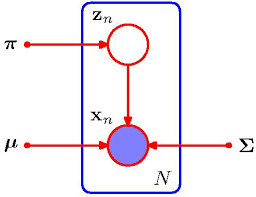
\includegraphics[scale=0.4]{./images/gmm.png}
	\end{center}
	\caption{Graphical representation of GMM model. The GMM models a joint distribution $p(\mathbf{x}, \mathbf{z})$ in terms of a marginal distribution $p(\mathbf{z})$ and conditional distribution $p(\mathbf{x}|\mathbf{z})$ to model $p(\mathbf{x})$. Each $\mathbf{x}_n$ is coupled with $\mathbf{z}_n$}
	\label{fig:gmm}
\end{figure}
Now we can work with the joint distribution $p(\mathbf{x,z})$ instead of the marginal distribution $p(\mathbf{x})$, which is hard to estimate directly as explained in \Cref{sec:intro_motivation}. 

Another quantity which plays a central role is the conditional proability of $\mathbf{z}$ given $\mathbf{x}$, $p(z_k=1|\mathbf{x})$. 
\begin{itemize}
\item $p(z_k=1) = \pi_k$ can be viewed as a prior of $z_k=1$
\item $\gamma(z_k)$: assignment probability or responsibility. This quantity will be updated through the Bayes Theorem.
\item[] $\rightarrow$  A simple explanation is that this is the classification result of $\mathbf{x}_n$.
\end{itemize}
\begin{align*}
\gamma(z_k) \equiv p(z_k=1|\mathbf{x}) & \equiv \frac{p(z_k=1)p(\mathbf{x}|z_k=1)}{\sum_{j=1}^{K}p(z_j=1)p(\mathbf{x}|z_j=1)} \\
& = \frac{\pi_k\mathcal{N}(\mathbf{x}|\boldsymbol{\mu}_k, \boldsymbol{\Sigma}_k)}{\sum_{j=1}^{K} \pi_j\mathcal{N}(\mathbf{x}|\boldsymbol{\mu}_j, \boldsymbol{\Sigma}_j)}
\end{align*}

\subsection{Maximum Likelihood}
Suppose we have a data set of observations $\mathbf{X}=\{\mathbf{x}_1,...,\mathbf{x}_n\}^{T}\in\mathbbm{R}^{N\times D}$ and we want to model the data distribution $p(\mathbf{X})$ using GMM. If we assume an \textrm{i.i.d.} data set, it can be expressed as follows: 
\begin{align*}
p(\mathbf{X}|\boldsymbol{\pi},\boldsymbol{\mu},\boldsymbol{\Sigma}) &=\prod_{n=1}^{N}\Bigg(\sum_{k=1}^{K}\pi_k\mathcal{N}(\mathbf{x}_n|\boldsymbol{\mu}_k, \boldsymbol{\Sigma}_k)\Bigg)\\
\end{align*}
then its loglikelihood function is given by:
\begin{align*}
\ln p(\mathbf{X}|\boldsymbol{\pi},\boldsymbol{\mu},\boldsymbol{\Sigma}) &= \sum_{n=1}^{N}\ln \Bigg(\sum_{k=1}^{K}\pi_k\mathcal{N}(\mathbf{x}_n|\boldsymbol{\mu}_k, \boldsymbol{\Sigma}_k)\Bigg)
\end{align*}

%In a single dimension case, 
%\begin{align*}
%	\ln p(x, \pi, \mu, \sigma) & =\sum_{n=1}^{N}\ln \sum_{k=1}^{K}\pi_k \frac{1}{\sigma_k \sqrt{2\pi_k}}\exp\Big(-\frac{1}{2}\Big(\frac{x_n-\mu_k}{\sigma_k}\Big)^2\Big)\\
%	\frac{\partial }{\partial \mu_k}\ln p(x, \pi, \mu, \sigma) & =\sum_{n=1}^{N} \frac{\pi_k \frac{1}{\sigma_k \sqrt{2\pi}}\exp\Big(-\frac{1}{2}\Big(\frac{x_n-\mu_k}{\sigma_k}\Big)^2\Big) \frac{x_n-\mu_k}{\sigma_k^2}}{\sum_{k=1}^{K}\pi_k \frac{1}{\sigma_k \sqrt{2\pi}}\exp\Big(-\frac{1}{2}\Big(\frac{x_n-\mu_k}{\sigma_k}\Big)^2\Big)}\\
%	& =\sum_{n=1}^{N} \underbrace{\frac{\pi_k \mathcal{N}(x_n|\mu_k, \sigma_k) }{\sum_{k=1}^{K}\pi_k \mathcal{N}(x_n|\mu_k, \sigma_k)}}_{=\gamma(z_{nk})}\frac{x_n-\mu_k}{\sigma_k^2}\\
%	\mu_k &=\frac{1}{N_k}\sum_{n=1}^{N} \gamma(z_{nk}) x_n,
%\end{align*}
%where 
%$N_k = \sum_{n=1}^{N} \gamma(z_{nk})$. $N_k$ can be interpreted as the effective number of points assigned to cluster $k$. 

Before, maximizing the likelihood, it is worth to emphasize two issues in GMM: (i) \textit{singularities} and (ii) \textit{identifiability}.

%\subsection{Singularity and Identifiability}
\paragraph{Singularity}
Suppose that one of the components of the mixture model, let us say the $j$-th component, has its mean $\mathbf{\mu}_j$ exactly equal to one of the data points so that $\mathbf{\mu}_j=\mathbf{x}_n$ for some value of $n$. This data point will then contributes a term in the likelihood function of the form 
$$\mathcal{N}(\mathbf{x}_n, \sigma_j^2\mathbf{I}) = \frac{1}{(2\pi)^{1/2}} \frac{1}{\sigma_j}$$
If we consider the limit $\sigma_j \to 0$, then we see that this term goes to infinity and so the log likelihood function will also go to infinity. Thus the maximization of the log likelihood function will also go to infinity. Thus the maximization of the log likelihood function is not a well posed problem because such sigularities will walways be present and will occur whenever one of the Gaussian components collapses onto a specific data point. 

\paragraph{Identifiability}
A further issue in finding MLE based solutions arises from the fact that for any given maximum likelihood solution, a $K$-component mixture will have a total ok $K!$ equivalent solutions corrsponding to the $K!$ ways of assigning $K$ sets of parameters to $K$ components. In other words, for any given point in the space of parameter values there will be a further $K!-1$ additional points all of which give rise to exactly the same distribution. 

\subsection{Expectation Maximization for GMM}

The goal of Expectation Maximization (EM) is to find maximum likelihood solutions for models having latent variables 
\begin{itemize}
	\item Suppose that it is hard to optimize $p(\mathbf{X}|\boldsymbol{\theta})$ directly.
	\item However, it is easier to optimize the complete-data likelihood function $p(\mathbf{X}, \mathbf{Z}|\boldsymbol{\theta})$ 
	\item In this case, we can use \textbf{EM algorithm}. EM algorithm is a general technique for finding maximum likelihood solutions for latent variable models. 
\end{itemize}

\begin{algorithm}
	Initialize the means $\boldsymbol{\mu}_k$, covariances $\boldsymbol{\Sigma}_k$ and mixing coefficients $\pi_k$ and evaluate the initial value of the log likelihood.\\
	\For{n}{
		E step: evaluate the responsibilities of $\mathbf{x}_n$ based on the current parameter values with the given parameters
		$$ \gamma(z_{nk})= p(z_k=1|\mathbf{x}_n) =  \frac{\pi_k\mathcal{N}(\mathbf{x}_n|\boldsymbol{\mu}_k, \boldsymbol{\Sigma}_k)}{\sum_{j=1}^{K} \pi_j\mathcal{N}(\mathbf{x}_n|\boldsymbol{\mu}_j, \boldsymbol{\Sigma}_j)}$$\\
		where $z_{nk}$ denote the $k$-th component of $\mathbf{z}_n$\\
		M step: maximize expectation
		\begin{itemize}
			\item $\boldsymbol{\mu}_k^{\textrm{new}} = \frac{1}{N_k}\sum_{n=1}^{N}\gamma(z_{nk})\mathbf{x}_n$
			\item $\boldsymbol{\Sigma}_k^{\textrm{new}} = \frac{1}{N_k}\sum_{n=1}^{N}\gamma(z_{nk})(\mathbf{x}_n-\boldsymbol{\mu}_k^{\textrm{new}})(\mathbf{x}_n-\boldsymbol{\mu}_k^{\textrm{new}})^T$
			\item $\pi_k^{\textrm{new}} = p(z_k=1) = \frac{N_k}{N}$
		\end{itemize}
	Evaluate the log likelihood to check for convergence of parameters
	$$\textrm{ln}p(\mathbf{X}|\boldsymbol{\pi},\boldsymbol{\mu},\boldsymbol{\Sigma}) = \sum_{n=1}^{N}\textrm{ln}\Bigg(\sum_{k=1}^{K}\pi_k\mathcal{N}(\mathbf{x}_n|\boldsymbol{\mu}_k, \boldsymbol{\Sigma}_k)\Bigg)$$
	}
	\caption{EM algorithm for GMM}
\end{algorithm}
	\begin{figure}[h]
	\begin{center}
		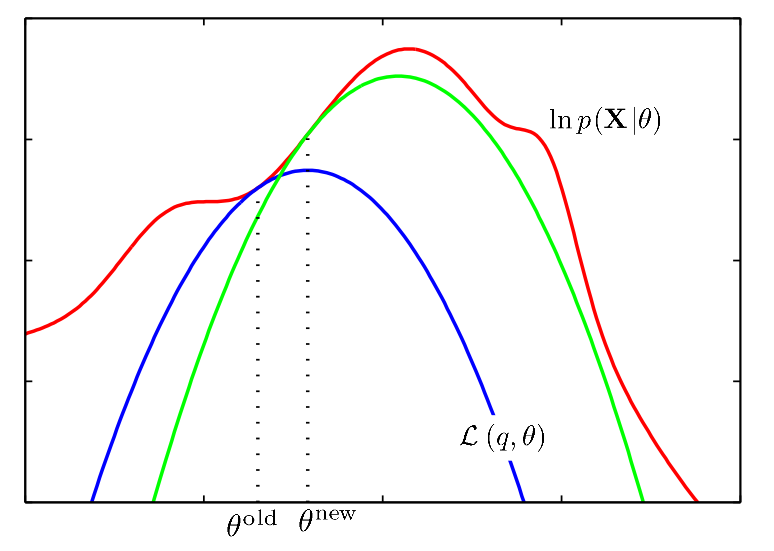
\includegraphics[scale=0.3]{./images/em_update.png}
	\end{center}
	\caption{M-step of EM algorithm}
	\label{fig:em2}
\end{figure}
